\section*{Dati e risultati}

\subsection*{Premessa}

In elettronica digitale ricordiamo che alla tensione continua di \SI{+5}{\volt} corrisponde il valore di verità 1, ovvero positivo. Mentre ad una tensione continua di \SI{0}{\volt} corrisponde il valore di verità 0, ovvero falso.

\subsection*{Porta NAND}

In questo paragrafo vogliamo verificare il corretto funzionamento di una porta NAND. Questa porta, intuitivamente non è altro che una porta AND la cui uscita è negata, ovvero è come se vi fosse un NOT all'uscitta della porta AND.
Quindi dalla teoria sappiamo che se denotiamo con A e B gli stati di ingresso di una porta logica e con O lo stato di uscita della stessa, la tabella di verità per la porta NAND risulta essere quella riportata in Tabella \ref{tab:nand}.

\begin{wrapfloat}{table}{I}{200pt}
\centering
	\begin{tabular}{lll}
	\toprule
		A & B & O \\
	\midrule
		0 & 0 & 1 \\
		0 & 1 & 1 \\
		1 & 0 & 1 \\
		1 & 1 & 0 \\
	\bottomrule
	\end{tabular}
	\caption{Tabella di verità della porta ogica NAND.}
	\label{tab:nand}
\end{wrapfloat}

Operativamente noi abbiamo fatto quanto segue: abbiamo collegato le alimentazioni $V\ped{cc}^+$ e $V\ped{cc}^-$ del circuito integrato SN74LS00N a \SI{+5}{\volt} e al comune (\SI{0}{\volt}) rispettivamente. Ricordiamo che tale circuito integrato presenta ben quattro porte NAND sullo stesso chip. Successivamente abbiamo collegato l'uscita della porta logica usata alla schedina LED e abbiamo verificato, variando i valori di tensione (\SI{+5}{\volt} e \SI{0}{\volt}) ai capi degli ingressi A e B, che la tablla di verità ottenuta corrispondesse con quella teorica.
Il risultato, come previsto, è stata la corretta corrispondenza tra teoria e pratica. Inoltre abbiamo osservato come in uscita dalla porta logica la tensione ($V\ped{out}$) fosse di \SI{+3}{\volt}.

\subsection*{Porta NOT}

In questa sezione vogliamo verificare il corretto funzionamento di una porta logica NOT. Innanzitutto abbiamo sfruttato il circuito integrato SN74LS00N per realizzare tale porta. Dal momento che l'SN74LS00N è una NAND, al fine di ottenere da tale porta logica un NOT, non dobbiamo fare altro che collegare entrambi gli ingressi allo stesso potenziale. Vedi Figura \ref{fig:not}

Detto questo sfruttando l'integrato SN74LS00N abbiamo collegato i suoi due ingressi al generatore di funzioni d'onda, e gli abbiamo dato in imput un'onda quadra di frequenza $f=\SI{2}{\hertz}$, di ampiezza \SI{5}{\volt} picco picco e con un offset di \SI{2.5}{\volt}.
Quindi siamo andati a verificarne il corretto funzionamento sulla schedina LED, collegata all'uscita della porta logica in esame. Quello che abbiamo osservato è che se in ingresso la tensione è \SI{+5}{\volt}, quindi 1 logico, in uscita si ottiene 0, mentre se in ingresso la tensione è di \SI{0}{\volt}, quindi lo 0 logico, in uscita si ottiene 1. Il risultato è pertanto corretto.% Inoltre abbiamo anche visualizzato, grazie all'oscilloscopio, l'andamento della tensione in ingresso alla porta logica $V\ped{in}$ e l'andamento di $V\ped{out}$, tensione in uscita dalla porta. Quello che abbiamo ottenuto è riportato in Figura \ref{fig:not_plot}.

\begin{SCfigure}[.90][h!]
    \centering
    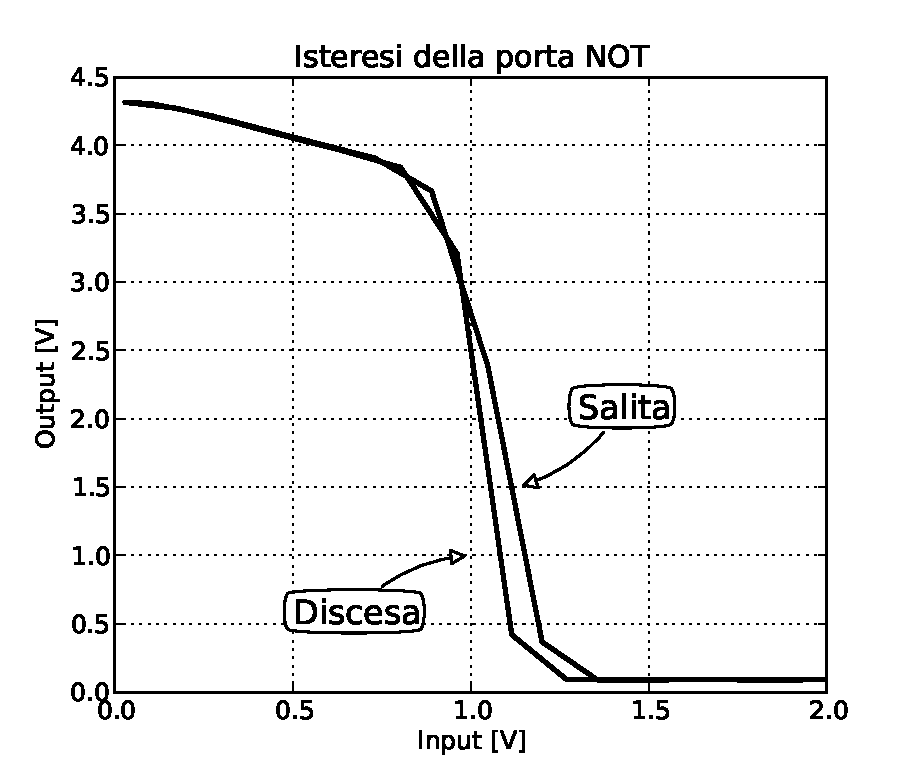
\includegraphics[width=0.55\columnwidth]{ist.pdf}
    \caption{Il grafico mostra l'isteresi della porta NOT. L'ampiezza dell'isteresi è di circa 0.1 V e avviene attorno alla tensione di input di valore \SI{1.1}{\volt}. Questo significa che partendo da \SI{0}{\volt} e salendo in tensione, si ha la commutazione tra i due stati logici a circa \SI{1.15}{\volt}, mentre scendendo da \SI{5}{\volt} la commutazione avviene a circa \SI{1.05}{\volt}. Come è possibile osservare la tensione alta non è sempre 5 V, anzi in base alla tensione di ingresso l'outut varia visibilmente. Questo è uno dei motivi per cui in elettronica digitale si lascia una certa tolleranza ai valori di tensione sia in ingresso che in uscita, dal momento che nessun componente è ideale.}
    \label{fig:not_tensioni}
\end{SCfigure}

Successivamente abbiamo studiato la variazione della tensione in uscita dalla porta logica $V\ped{out}$ al variare della tensione in ingresso $V\ped{in}$ della stessa. La tensione in ingresso è stata variata partendo da una tensione di \SI{0}{\volt} fino ad arrivare ad una tensione di \SI{+5}{\volt}, e viceversa, partendo da \SI{+5}{\volt} e arrivando a \SI{0}{\volt}. Quello che abbiamo ottenuto è riportato nel grafico in Figura \ref{fig:not_tensioni}.

\subsection*{Porta AND}

L'obbiettivo di questa sezione è quello di realizzare una porta AND sfruttando solo la porta logica NAND. A tal fine abbiamo usato l'integrato SN74LS00N alimentato nello stesso modo descritto nella sezione sulla porta NAND.
Quindi abbiamo realizzato il circuito descritto in Figura \ref{fig:and}. Ovvero con una prima porta logica NAND con due ingressi A e B abbiamo ottenuto un AND negato. Quindi al fine di ottenere un AND dobbiamo solamente negare nuovamente l'uscita $V\ped{O1}$. Per fare questo poniamo il segnale in uscita $V\ped{O1}$ ad entrambi gli ingresso di una nuova porta NAND, in questo modo questa funziona come NOT in quanto i segnali in ingresso sono gli stessi.

Quindi sfruttando l'osciloscopio abbiamo verificato che l'uscita del secondo NAND risultasse uguale all'uscita di una porta AND.

Possiamo inoltre immaginare la porta AND come un'interruttore. Infatti mantenendo uno dei due ingressi A o B ad una tensione di \SI{+5}{\volt}, quindi 1 logico, possiamo decidere se far passare o meno un segnale semplicemente agendo sull'ingresso libero.
Quindi se per esempio A è fisso ad 1 logico, in base al valore di B oteniamo una trasmissione del seganle o un'interruzione del segnale. Quindi A si può pensare come ad una linea dati e B come ad un vero e proprio interruttore che se è collegato ad una tensione di \SI{+5}{\volt} permette il passaggio del segnale, mentre se è collegato al conune \SI{0}{\volt} non permette il passaggio del seganle.

Infine osserviamo come in algebra di Boole tale porta rappresenti l'operazione di moltiplicazione. Questa analogia ci tornrà utile nel momento in cui si dovranno relizzare dei circuiti a partire dall'analisi di una tabella di verità o dallo studio della funzione di uscita del circuito che si vuole realizzare.

\subsection*{Porta XOR}

In questa sezione vogliamo realizzare una porta XOR utilizzando solamente delle porte NAND. La tabella di verità di una porta XOR è la seguente:
\begin{center}
	\begin{tabular}{lll}
	\toprule
		A & B & C \\
	\midrule
		0 & 0 & 0 \\
		0 & 1 & 1 \\
		1 & 0 & 1 \\
		1 & 1 & 0 \\
	\bottomrule
	\end{tabular}
\end{center}
La configurazione circuitale che abbiamo adotato al fine di realizare una XOR con solo porte NAND è raffigurata in Figura \ref{fig:xor}. La tabella di verità di questo circuito è la seguente:
\begin{center}
	\begin{tabular}{llllll}
	\toprule
		A & B & C & D & E & F \\
	\midrule
		0 & 0 & 1 & 1 & 1 & 0 \\
		0 & 1 & 1 & 1 & 0 & 1 \\
		1 & 0 & 1 & 0 & 1 & 1 \\
		1 & 1 & 0 & 1 & 1 & 0 \\
	\bottomrule
	\end{tabular}
\end{center}
Tale caratteristica di uscita del nosto circuito è stata verificata grazie alla schedina LED, che ci ha permesso di accertarci che effettivamente quando i due ingressi A e B sono differenti tra di loro l'uscita si trova ad 1 logico, mentre quando sono uguali l'uscita è allo 0 logico.

\subsection*{Votazione}

In questa sezione vogliamo cercare di realizzare un sistema che presi in input i valori d verità di 3 giurati e 1 presisdente, quindi 4 elementi, restituisca in output il risultato della votazione. Ovvero restituisca 1 se la votazione ha avuto esito positivo, 0 se la votazione ha avuto esito negativo. Inoltre occorre tenere presente, ai fini della realizzazione, che il voto del presidente ha un peso doppio rispetto a quello degli altri giurati. Naturalmente un voto favorevole ha valore di verità pari ad 1, mentre uno contrario ha valore pari a 0.

Quindi per ralizzare tale circuito come prima cosa dobbiamo creare la tabella di verità. Questa è riportata in Tabella \ref{tab:votazione}.

\begin{wrapfloat}{table}{I}{250pt}
\centering
\begin{tabular}{l c c c | l}
	\toprule
		P & A & B & C & O \\
	\midrule
		0 & 0 & 0 & 0 & 0 \\
		0 & 0 & 0 & 1 & 0 \\
		0 & 0 & 1 & 0 & 0 \\
		0 & 0 & 1 & 1 & 0 \\
		0 & 1 & 0 & 0 & 0 \\
		0 & 1 & 0 & 1 & 0 \\
		0 & 1 & 1 & 0 & 0 \\
		0 & 1 & 1 & 1 & 1 \\
		1 & 0 & 0 & 0 & 0 \\
		1 & 0 & 0 & 1 & 1 \\
		1 & 0 & 1 & 0 & 1 \\
		1 & 0 & 1 & 1 & 1 \\
		1 & 1 & 0 & 0 & 1 \\
		1 & 1 & 0 & 1 & 1 \\
		1 & 1 & 1 & 0 & 1 \\
		1 & 1 & 1 & 1 & 1 \\
	\bottomrule
\end{tabular}
\caption{Tabella di verità della votazione.}
\label{tab:votazione}
\end{wrapfloat}

La Tabella \ref{tab:votazione} rappresenta la tabella di verità del nostro sistema di votazione.
P indica il voto del presidente. A, B, C i voti dei giurati. O il risultato della votazione. Ricordiamo che 1 = voto favorevole, mentre 0 = voto contrario.
Come è possibile osservare, dal momento che il presisdente di giuria ha un peso doppio rispetto agli altri giurati, se il suo verdetto è negativo (0) il risultato della votazione è anch'esso negativo (0) a meno che tutti e tre i guirati non esprimano un voto favorevole (1). In questo caso la votazione avrebbe esito positivo (1). Al contrario se il presidente esprime un consenso ovvero 1 allora il risutato della votazione sarà sempre favorevole (1). Anche in questo caso l'unica eccezzione è se tutti i giurati esprimono un foto sfavorevole (0). In questo caso la votazione avrà esito negativo, 0.
Quindi per realizzare il circuito dobbiamo trovare la funzione di uscita dello stesso. Per farlo sfruttiamo la mappa di Karnaugh e le leggi di De Morgan. Quindi abbiamo che, se con Y indichiamo l'uscita del nostro circuito, questa è data da:

\begin{equation*}
	Y\,=\,PC+PA+ABC 
\end{equation*}

Quindi sfruttando le leggi di De Morgan che ci dicono che:

\begin{equation*}
	\overline{A+B}\,=\,\overline{A} \cdot \overline{B} \qquad \text{e} \qquad \overline{A \cdot B}\,=\,\overline{A}+\overline{B}
\end{equation*}

otteniamo il seguente risultato:

\begin{equation}
	Y\,=\, \overline{ \overline{PC \cdot PA} \cdot \overline{ABC} }
\label{eq:Y_votazione}
\end{equation}

Quindi dall'equazione (\ref{eq:Y_votazione}) possiamo dedurre che per realizzare il circuito ci occorrono solamente delle porte NAND, infatti ricordiamoci che una porta NOT può essere ottenuta grazie ad una porta NAND, come abbiamo già visto. Quindi a questo punto siamo in grado di realizzare il nostro circuito per la votazione. Infatti ricordandoci che l'operazione di moltiplicazione, in algebra di Boole, è associata alla porta logica AND e l'operazione di somma è associata alla porta logica OR, sfruttando la doppia negazione possiamo ricondurci alle porte logiche NAND e NOT analizzate in precedenza. Il risultato è illustrato in Figura \ref{fig:votazione}.

\begin{figure}[h!]
    \centering
    \begin{circuitikz}[scale=0.65, transform shape]
        % Parte sopra
        \draw
        (2, 3) node[american nand port] (nand1A) {}
        (2, 1) node[american nand port] (nand1B) {}
        (4, 2) node[american nand port] (nand1C) {}
        (5, 2) node[american not port] (not1) {}
        (nand1A.out) -| (nand1C.in 1)
        (nand1B.out) -| (nand1C.in 2)
        (nand1C.out) -- (not1.in)
        (nand1A.in 2) -- ++(-2,0) node[left]{A}
        (nand1B.in 2) -- ++(-2,0) node[left]{B}
        (nand1A.in 1) ++(-2,0) node[left]{P} -| (nand1B.in 1)
        ;
        
        % Prima parte sotto
        \draw
        (2, -1) node[american nand port] (nand2) {}
        (2, -3) node[american not port] (not2) {}
        (nand1A.in 1) ++(-0.3,0) |- (nand2.in 1)
        (nand1B.in 2) ++(-0.6,0) |- (nand2.in 2)
        (nand1A.in 1) ++(-0.9,0) |- (not2.in)
        ;
         
        % Seconda parte sotto
        \draw
        (4.5, -2) node[american nand port] (nand3A) {}
        (6.5, -3) node[american nand port] (nand3B) {}
        (nand2.out) -| (nand3A.in 1)
        (not2.out) -| (nand3A.in 2)
        (nand3A.out) -| (nand3B.in 1)
        (nand3B.in 2) -- ++(-1,0) node[left]{C}
        ;
        
        % Unione
        \coordinate (U) at ($ (nand3B.out) !0.5! (not1.out) $); % !0.5! moltiplica per 0.5
        \draw
        (U) ++ (3,0) node [american nand port] (nand4) {}
        (not1.out) -| (nand4.in 1)
        (nand3B.out) -| (nand4.in 2)
        (nand4.out) -- ++(0.5,0) node[right]{OUT}
        ;
    \end{circuitikz}
    \caption{}
    \label{fig:votazione}
\end{figure}

\subsection*{Allarme}

In quest'ultima sezione vogliamo cercare di realizzare un semplice sistema di allarme. Prendiamo in considerazione i seguenti sensori:
\begin{itemize}\itemsep2pt \parskip0pt \parsep0pt
	\item{P: sensore posto sulla porta di igresso. 0 = chiusa, 1 = aperta;}
	\item{F: sensore posto sulla finestra. 0 = chiusa, 1 = aperta;}
	\item{I: sensore infrarossi interno all'appartamento. 0 = non rileva persone, 1 = rileva persone;}
	\item{C: chiave che esclude il sistema di infrarossi (I). 1 = sistema infrarosso non in funzione;}
\end{itemize}
Quindi in modo analogo a quanto fatto per la progettazione del sistema di votazione andiamo a realizzare la tabella di verità di questo circuito. La tabella di verità è riportata in Tabella \ref{tab:allarme}.

\begin{wrapfloat}{table}{I}{250pt}
\centering
\begin{tabular}{l c c c | l}
	\toprule
		P & F & I & C & O \\
	\midrule
		0 & 0 & 0 & 0 & 0 \\
		0 & 0 & 0 & 1 & 0 \\
		0 & 0 & 1 & 0 & 1 \\
		0 & 0 & 1 & 1 & 0 \\
		0 & 1 & 0 & 0 & 1 \\
		0 & 1 & 0 & 1 & 1 \\
		0 & 1 & 1 & 0 & 1 \\
		0 & 1 & 1 & 1 & 1 \\
		1 & 0 & 0 & 0 & 1 \\
		1 & 0 & 0 & 1 & 1 \\
		1 & 0 & 1 & 0 & 1 \\
		1 & 0 & 1 & 1 & 1 \\
		1 & 1 & 0 & 0 & 1 \\
		1 & 1 & 0 & 1 & 1 \\
		1 & 1 & 1 & 0 & 1 \\
		1 & 1 & 1 & 1 & 1 \\
	\bottomrule
\end{tabular}
\caption{Tabella di verità dell'allarme.}
\label{tab:allarme}
\end{wrapfloat}

La Tabella \ref{tab:allarme} illusta il sistema di funzionamento del nostro circuito. Ovvero, se momentaneamente non si considea la chiave, abbiamo che basta un solo segnale di P, F o I positivo, ovvero 1, che il sistema di allarme scatta. Quindi se denotiamo con O l'uscita del circuito questa avrà valore di verità 1. Nel momento in cui la chiave (C) è inserita (1) questa va a sostituirsi al sistema ad infrarosso. Infatti come si può notare se P o F sono positivi (1), a chaive inserita, il sistema di allarme scatta (1). Al contario se P o F sono negativi (0), achiave inserita, il sistema di allarme non scatta (0). Infine quando la chiave è disinserita (0) questa può essere trascurata e quindi si ritorna al caso iniziale, ovvero come se C non esistesse.

Quindi anche in questo caso per realizzare il circuito dobbiamo studiare la funzione di uscita del circuito (Y). Per farlo ci avvaliamo ancora una volta della mappa di Karnaugh e delle leggi di De Morgan. Pertanto la funzione di uscita risulta essere:

\begin{equation*}
	Y\,=\,I\overline{C} + F + P
\end{equation*} 

Quindi grazie alle leggi di De Morgan otteniamo che:

\begin{equation}
	Y\,=\,I\overline{C} \cdot FP
	\label{eq:Y_allarme}
\end{equation}

\begin{wrapfloat}{figure}{O}{350pt}
    \centering
        \begin{circuitikz}
            \draw
                (1.8, 0) node[nand port] (nand1) {}
				(1.8, 2) node[nand port] (nand2) {}
				(1.8, 4) node[nand port] (nand3) {}
				(0, 0) node[anchor=east] {F} -| (nand1.in 1)
				(0, 0) -| (nand1.in 2)
				(0, 2) node[anchor=east] {P} -| (nand2.in 1)
				(0, 2) -| (nand2.in 2)
				(0, 4) node[anchor=east] {C} -| (nand3.in 1)
				(0, 4) -| (nand3.in 2)
				(3.5, 5) node[nand port] (nand4) {}
				(3.5, 1) node[nand port] (nand5) {}
				(5, 1) node[nand port] (nand6) {}
				(nand1.out) -| (nand5.in 2)
				(nand2.out) -| (nand5.in 1)
				(0, 6) node[anchor=east] {I} -| (nand4.in 1)
				(nand3.out) -| (nand4.in 2)
				(nand5.out) -| (nand6.in 1)
				(nand5.out) -| (nand6.in 2)
				(7, 3) node[nand port] (nand7) {}
				(nand6.out) -| (nand7.in 2)
				(nand4.out) -| (nand7.in 1)
				(nand7.out) node[anchor=west] {OUT}
            ;
        \end{circuitikz}
    \caption{}
    \label{fig:allarme}
\end{wrapfloat}

Quindi grazie all'equazione (\ref{eq:Y_allarme}) noi sappiamo che ci occorrono 3 porte NAND e 4 porte NOT per realizzare il circuito desiderato. Infatti basta ricordarsi che per realizzare un AND occorre un NAND la cui uscita deve essere negata con un NOT. Questo è un risultato ottenuto nella sezione relativa all'analisi della porta NAND. Inoltre se si folesse usare solamente la porta NAND, invece che NAND e NOT basta ricordarsi che una NAND può essere vista come un NOT, basta collegare entrambi gli inressi della NAND allo stesso segnale. Quindi grazie a queste informazioni abbiamo realizzato il circuito in Figura \ref{fig:allarme}.



%\begin{wrapfloat}{figure}{I}{0pt}
%\includegraphics[width=0.5\textwidth]{Relativo}
%\caption{Esempio di figura ‘‘avvolta’’ da un testo.}
%\end{wrapfloat}

%\begin{center}
%	\begin{tabular}{lll}
%	\toprule
%		A & B & C \\
%	\midrule
%		& & \\
%		& & \\
%		& & \\
%		& & \\
%	\bottomrule
%	\end{tabular}
%\end{center}

%\begin{figure}[t!]
%    \centering
%    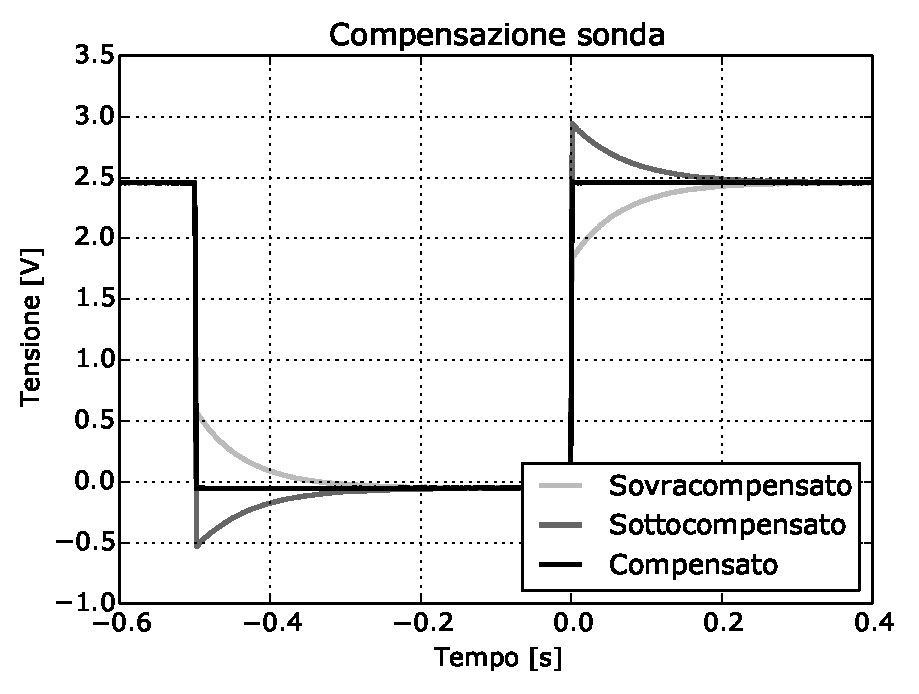
\includegraphics[width=\columnwidth]{figure/comp.pdf}
%    \caption{Input dell'oscilloscopio con una sonda compensabile. Cambiando capacità
%        si può ottenere una sottocompensazione, una sovracompensazione oppure compensare perfettamente
%        le capacità, ottenendo un'onda quadra.}
%    \label{fig:compensazione}
%\end{figure}

%\begin{wrapfloat}{figure}{O}{0pt}
%        \def\svgwidth{0.4\textwidth}
%        \subimport{figure/}{raddrizzatore.pdf_tex}
%        \caption{Raddrizzatore di precisione a semionda. Alimentato, inizialmente con una $V\ped{in}\,=\,\SI{1.02}{\volt}$ di frequenza $\nu\,=\,\SI{50}{\hertz}$.}
%        \label{fig:radd}
%\end{wrapfloat}

%\begin{SCfigure}[][p]
%        \centering
%        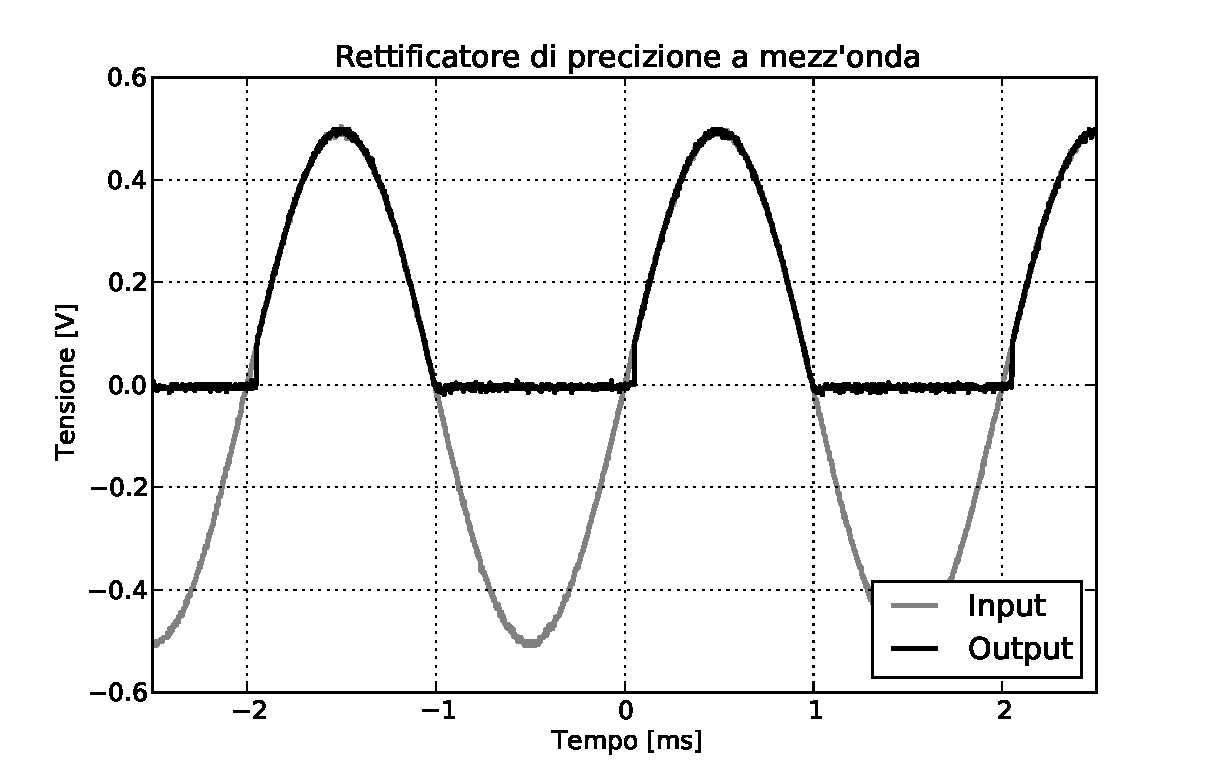
\includegraphics[width=0.7\textwidth]{figure/rett.pdf}
%        \caption{Questo grafico illustra l'andamento di $V\ped{out}$, linea nera, in funzione di $V\ped{in}$, linea grigia. Si nota chiaramente, come da previsioni, che la parte negativa del segnale in ingresso impediscse al diodo di condurre, pertanto la tensione di output risulta nulla. Inoltre, come si può osservare, il fronte di salita di $V\ped{out}$ presenta un leggero ritardo rispetto al segnale in ingresso $V\ped{in}$. Questo ritardo è stato stimato essere approssimativamente di circa $(152\pm10)\SI{}{\micro\second}$.}
%        \label{fig:radd_plot1}
%\end{SCfigure}
